% FinalPresentation.tex
% EE133/233 FM Radio Receiver -- Final Project Presentation
% Students: Edison Altamirano (006948159), Sahan (006948160)
% Compiler: pdflatex
% NOTE: run MatlabSimulations/generate_plots.py ONCE before compiling
%       to produce the image files referenced in Slides 8-10.

\documentclass[aspectratio=169]{beamer}
\usetheme{CambridgeUS}
\usecolortheme{beaver}

\usepackage{tikz}
\usetikzlibrary{arrows.meta,shapes.geometric,positioning,calc,
                decorations.pathmorphing,patterns}
\usepackage{pgfplots}
\pgfplotsset{compat=1.18}
\usepackage{amsmath,amssymb}
\usepackage{graphicx}
\usepackage{xcolor}
\usepackage{colortbl}
\usepackage{booktabs}

%% ── Color palette ───────────────────────────────────────────────────────────
\definecolor{rfcol}{RGB}{200,30,30}
\definecolor{ifcol}{RGB}{20,80,200}
\definecolor{bbcol}{RGB}{10,150,60}
\definecolor{locol}{RGB}{130,0,150}
\definecolor{blkbg}{RGB}{30,80,160}
\definecolor{gblk} {RGB}{50,160,80}
\definecolor{yblk} {RGB}{255,220,50}

%% ── TikZ styles (defined in preamble to avoid Beamer #1 conflict) ──────────
\tikzset{
  blkmain/.style ={draw, fill=#1, minimum width=1.4cm, minimum height=0.75cm,
                   align=center, font=\small\bfseries, rounded corners=2pt},
  blksmall/.style={draw=#1, fill=#1!15, minimum width=1.1cm, minimum height=0.45cm,
                   align=center, font=\tiny\bfseries},
  blkmed/.style  ={draw=#1, fill=#1!15, minimum width=1.3cm, minimum height=0.5cm,
                   align=center, font=\tiny\bfseries},
  arrcol/.style  ={-Stealth, line width=1.2pt, #1},
  arrthin/.style ={-Stealth, thick, #1},
  freqlab/.style ={font=\footnotesize\bfseries, #1},
}

\setbeamertemplate{navigation symbols}{}
\setbeamertemplate{footline}{}
\setbeamerfont{frametitle}{size=\large,series=\bfseries}

%% ============================================================
\begin{document}

%% ── SLIDE 1: TITLE ──────────────────────────────────────────────────────────
\begin{frame}
\begin{center}
  {\Large\bfseries\color{red} EE133/233 FM Radio Receiver}

  \vspace{0.3cm}
  {\large\color{red} System Overview --- Final Project}

  \vspace{1.2cm}
  {\large Edison Altamirano (006948159) \quad Sahan (006948160)}

  \vspace{0.6cm}
  {\small EE133/233 --- Stanford University}

  \vspace{0.6cm}
  {\large March 2026}
\end{center}
\end{frame}

%% ── SLIDE 2: FULL SYSTEM ARCHITECTURE ──────────────────────────────────────
\begin{frame}{Full System Architecture (1/2)}
\vspace{-0.1cm}
\begin{center}
\resizebox{0.97\textwidth}{!}{%
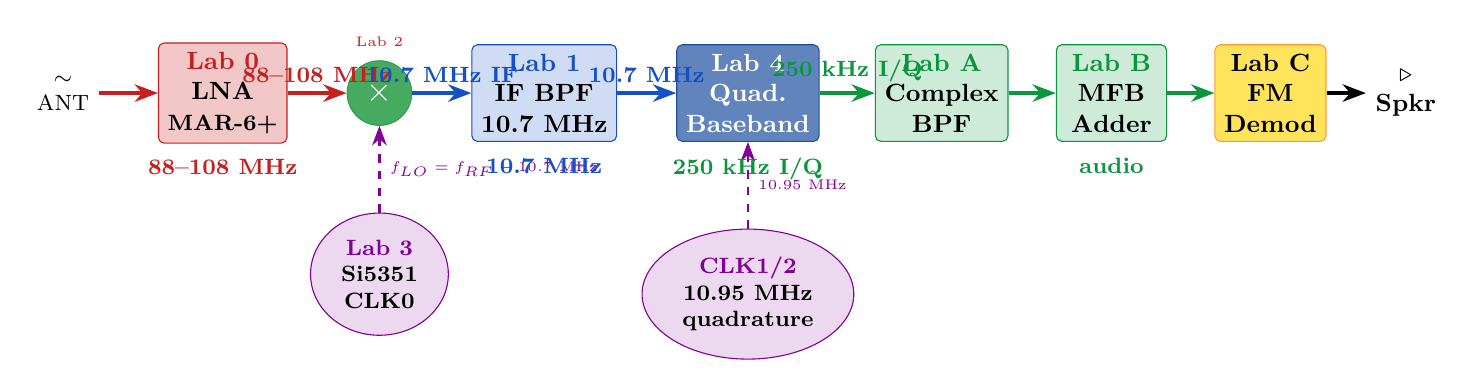
\begin{tikzpicture}[
  xblk/.style={draw=gblk, fill=gblk!90, circle, minimum size=0.82cm,
               font=\bfseries\large, text=white},
  lobox/.style={draw=locol, fill=locol!15, ellipse, minimum width=1.75cm,
                minimum height=0.78cm, align=center, font=\footnotesize\bfseries},
  larr/.style={-Stealth, dashed, line width=0.9pt, draw=locol},
  node distance=0.55cm
]
%% Main chain
\node[font=\footnotesize, align=center] (ant) {$\sim$\\ANT};

\node[blkmain=rfcol!25, draw=rfcol, right=0.75cm of ant] (lna1)
  {\textcolor{rfcol}{Lab 0}\\LNA\\\footnotesize MAR-6+};

\node[xblk, right=0.75cm of lna1] (mix)  {\textbf{$\times$}};
\node[font=\tiny, above=0.05cm of mix]{\textcolor{rfcol}{Lab 2}};

\node[blkmain=ifcol!20, draw=ifcol, right=0.75cm of mix] (bpf)
  {\textcolor{ifcol}{Lab 1}\\IF BPF\\10.7 MHz};

\node[draw=blkbg, fill=blkbg!70, minimum width=1.4cm, minimum height=0.75cm,
      align=center, font=\small\bfseries, rounded corners=2pt,
      right=0.75cm of bpf, text=white] (qb)
  {Lab 4\\Quad.\\Baseband};

\node[blkmain=bbcol!20, draw=bbcol, right=0.7cm of qb] (cbpf)
  {\textcolor{bbcol}{Lab A}\\Complex\\BPF};

\node[blkmain=bbcol!20, draw=bbcol, right=0.6cm of cbpf] (add)
  {\textcolor{bbcol}{Lab B}\\MFB\\Adder};

\node[blkmain=yblk!80, draw=orange!80, right=0.6cm of add] (dem)
  {Lab C\\FM\\Demod};

\node[right=0.5cm of dem, font=\small\bfseries, align=center] (spk)
  {$\triangleright$\\Spkr};

%% LO sources
\node[lobox, below=1.1cm of mix] (lo3)
  {\textcolor{locol}{Lab 3}\\Si5351\\CLK0};
\node[lobox, below=1.1cm of qb]  (lo01)
  {\textcolor{locol}{CLK1/2}\\10.95 MHz\\quadrature};

%% Main arrows
\draw[arrcol=rfcol]  (ant)  -- (lna1);
\draw[arrcol=rfcol]  (lna1) -- node[above,freqlab=rfcol]{\footnotesize 88--108 MHz} (mix);
\draw[arrcol=ifcol]  (mix)  -- node[above,freqlab=ifcol]{\footnotesize 10.7 MHz IF} (bpf);
\draw[arrcol=ifcol]  (bpf)  -- node[above,freqlab=ifcol]{\footnotesize 10.7 MHz} (qb);
\draw[arrcol=bbcol]  (qb)   -- node[above,freqlab=bbcol]{\footnotesize 250 kHz I/Q} (cbpf);
\draw[arrcol=bbcol]  (cbpf) -- (add);
\draw[arrcol=bbcol]  (add)  -- (dem);
\draw[arrcol=black]  (dem)  -- (spk);

%% LO arrows
\draw[larr] (lo3)  -- node[right,font=\tiny,locol]{$f_{LO}=f_{RF}-10.7$ MHz} (mix);
\draw[larr] (lo01) -- node[right,font=\tiny,locol]{10.95 MHz} (qb);

%% Freq labels below blocks
\node[freqlab=rfcol, below=0.08cm of lna1]{\footnotesize 88--108 MHz};
\node[freqlab=ifcol, below=0.08cm of bpf] {\footnotesize 10.7 MHz};
\node[freqlab=bbcol, below=0.08cm of qb]  {\footnotesize 250 kHz I/Q};
\node[freqlab=bbcol, below=0.08cm of add] {\footnotesize audio};

\end{tikzpicture}
}
\end{center}

\end{frame}

\begin{frame}{Full System Architecture (2/2)}
\begin{center}
\large\textbf{Signal Flow by Stage}
\end{center}
\vspace{0.25cm}
\begin{columns}[t]
\column{0.33\textwidth}
  \centering\textbf{\textcolor{rfcol}{RF Stage}}\\
  Antenna $\to$ LNA $\to$ Mixer\\
  88--108 MHz $\to$ 10.7 MHz
\column{0.33\textwidth}
  \centering\textbf{\textcolor{ifcol}{IF Stage}}\\
  IF BPF selects 10.7 MHz\\
  Image rejection + channel filtering
\column{0.33\textwidth}
  \centering\textbf{\textcolor{bbcol}{Baseband}}\\
  I/Q $\to$ Complex BPF $\to$ FM demod\\
  250 kHz $\to$ audio
\end{columns}
\vspace{0.3cm}
\begin{center}
\small\textbf{Core path:} 88--108 MHz RF $\rightarrow$ 10.7 MHz IF $\rightarrow$ 250 kHz low-IF $\rightarrow$ audio
\end{center}
\end{frame}

%% ── SLIDE 3: LAB 0 LNA ──────────────────────────────────────────────────────
\begin{frame}{Lab 0 --- MAR-6+ Low-Noise Amplifier (1/2)}
\textbf{What it does}

The MAR-6+ is the first stage amplifier.
It sets the noise floor for the entire receiver (Friis equation):
\[
  F_\text{sys} \approx F_1 + \frac{F_2 - 1}{G_1}
\]
With $G_1 \approx 22$ dB, noise from all later stages is suppressed by $\times 158$.

\vspace{0.3cm}
\begin{tabular}{ll}
\toprule
Parameter & Value \\
\midrule
IC        & MAR-6+ (Mini-Circuits) \\
Gain      & $\approx 22$ dB @ 100 MHz \\
NF        & 2.3 dB \\
Bandwidth & 1 MHz -- 1 GHz \\
Supply    & 5 V via bias-T \\
\bottomrule
\end{tabular}

\vspace{0.3cm}
\small Placed at the antenna input: boosts the weak FM signal before the mixer.\\[4pt]
Measured with NanoVNA S$_{21}$ + VAT-20+ attenuator on port 1.
\end{frame}

\begin{frame}{Lab 0 --- MAR-6+ Low-Noise Amplifier (2/2)}
\textbf{S$_{21}$ gain vs frequency (NanoVNA measurement)}
\begin{center}
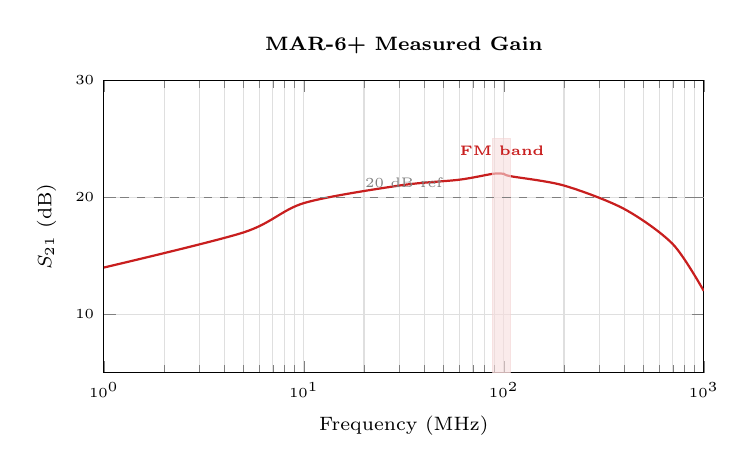
\begin{tikzpicture}
\begin{axis}[
  width=9.2cm, height=5.3cm,
  xlabel={Frequency (MHz)}, ylabel={$S_{21}$ (dB)},
  xmin=1, xmax=1000, xmode=log,
  xtick={1,10,100,1000},
  ymin=5, ymax=30,
  grid=both, grid style={gray!25},
  tick label style={font=\tiny},
  label style={font=\scriptsize},
  title={MAR-6+ Measured Gain}, title style={font=\scriptsize\bfseries},
]
  \addplot[rfcol, thick, smooth] coordinates {
    (1,14)(5,17)(10,19.5)(30,21)(60,21.5)
    (88,22)(100,22)(108,21.8)(200,21)
    (400,19)(700,16)(1000,12)};
  \addplot[rfcol!20, fill=rfcol!15, opacity=0.6]
    coordinates{(88,5)(88,25)(108,25)(108,5)} \closedcycle;
  \node[font=\tiny\bfseries,rfcol] at (axis cs:98,24){FM band};
  \draw[dashed,gray,thin](axis cs:1,20)--(axis cs:1000,20)
    node[midway,above,font=\tiny]{20 dB ref};
\end{axis}
\end{tikzpicture}
\end{center}

\vspace{0.1cm}
\begin{center}
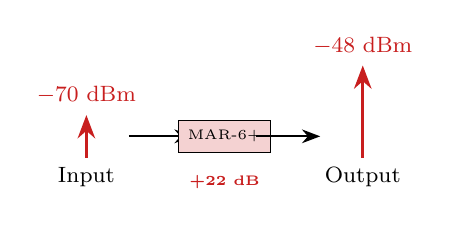
\begin{tikzpicture}[scale=0.9, every node/.style={font=\footnotesize}]
  \draw[rfcol,-Stealth,very thick](0,0)--(0,0.6)
    node[above]{\textcolor{rfcol}{$-70$ dBm}};
  \node[below] at (0,0){Input};
  \draw[-Stealth,thick](0.6,0.3)--(1.5,0.3);
  \node[draw,fill=rfcol!20,minimum width=0.9cm,minimum height=0.4cm]
    at (1.95,0.3){\tiny MAR-6+};
  \draw[-Stealth,thick](2.4,0.3)--(3.3,0.3);
  \draw[rfcol,-Stealth,very thick](3.9,0)--(3.9,1.3)
    node[above]{\textcolor{rfcol}{$-48$ dBm}};
  \node[below] at (3.9,0){Output};
  \node[rfcol,font=\tiny\bfseries] at (1.95,-0.35){+22 dB};
\end{tikzpicture}
\end{center}
\end{frame}

%% ── SLIDE 4: LAB 2 MIXER ────────────────────────────────────────────────────
\begin{frame}{Lab 2 --- ADE-1 Diode Ring Mixer: First Downconversion (1/2)}
\textbf{Frequency translation}
\begin{center}
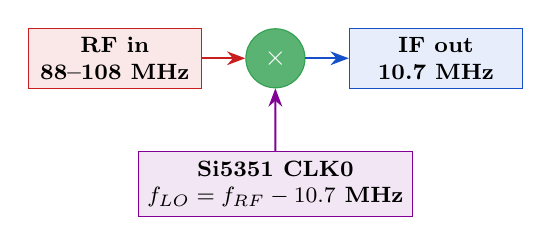
\begin{tikzpicture}[scale=0.95, every node/.style={font=\footnotesize}]
  \node[draw=rfcol,fill=rfcol!10,minimum width=2.2cm,minimum height=0.55cm,
        align=center,font=\footnotesize\bfseries] (rf){RF in\\88--108 MHz};
  \node[draw=gblk,fill=gblk!80,circle,minimum size=0.75cm,
        right=0.55cm of rf,font=\bfseries,text=white] (x){$\times$};
  \node[draw=ifcol,fill=ifcol!10,minimum width=2.2cm,minimum height=0.55cm,
        align=center,font=\footnotesize\bfseries,right=0.55cm of x] (ifb){IF out\\10.7 MHz};
  \node[draw=locol,fill=locol!10,minimum width=2.5cm,minimum height=0.55cm,
        align=center,font=\footnotesize\bfseries,below=0.8cm of x] (lo)
        {Si5351 CLK0\\$f_{LO}=f_{RF}-10.7$ MHz};
  \draw[-Stealth,rfcol,thick](rf)--(x);
  \draw[-Stealth,ifcol,thick](x)--(ifb);
  \draw[-Stealth,locol,thick](lo)--(x);
\end{tikzpicture}
\end{center}

\vspace{0.3cm}
\textbf{Example} (tuned to 98.1 MHz):
\[
  f_{LO} = 98.1 - 10.7 = \mathbf{87.4\text{ MHz}}
\]
\[
  f_{IF} = |f_{RF} - f_{LO}| = \mathbf{10.7\text{ MHz}}
\]

\vspace{0.3cm}
\textbf{Image frequency concern:}\\
Signal at $f_{img} = f_{LO} - 10.7 = 76.7$ MHz also mixes to 10.7 MHz.\\
IF BPF (Lab 1) must reject it before mixing.
\end{frame}

\begin{frame}{Lab 2 --- ADE-1 Diode Ring Mixer: First Downconversion (2/2)}
\textbf{Mixer output spectrum (RF = 98.1 MHz)}
\begin{center}
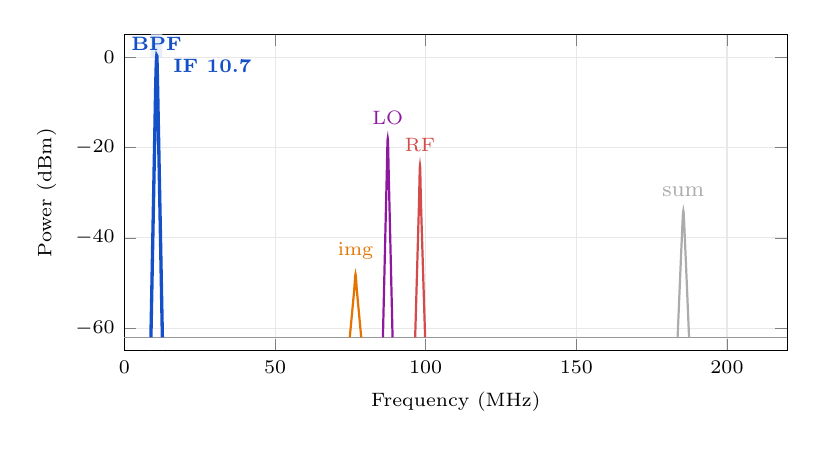
\begin{tikzpicture}
\begin{axis}[
  width=10.0cm, height=5.6cm,
  xlabel={Frequency (MHz)}, ylabel={Power (dBm)},
  xmin=0, xmax=220, ymin=-65, ymax=5,
  xtick={0,50,100,150,200},
  grid=both, grid style={gray!18},
  tick label style={font=\scriptsize},
  label style={font=\scriptsize},
  clip=false,
]
  \addplot[draw=none,fill=ifcol!10]
    coordinates{(8.8,-65)(8.8,5)(12.6,5)(12.6,-65)}\closedcycle;
  \node[ifcol,font=\scriptsize\bfseries] at (axis cs:10.7,3){BPF};
  \addplot[black!40,thin,smooth] coordinates{
    (0,-62)(50,-62)(100,-62)(150,-62)(200,-62)(220,-62)};
  \addplot[ifcol,very thick,smooth] coordinates{
    (8.8,-62)(10.0,-20)(10.4,-6)(10.7,0)(11.0,-6)(12.6,-62)};
  \node[ifcol,font=\scriptsize\bfseries,anchor=west] at (axis cs:13,-2){IF 10.7};
  \addplot[orange!90!black,thick,smooth] coordinates{
    (74.8,-62)(76.2,-52)(76.7,-48)(77.2,-52)(78.6,-62)};
  \node[orange!90!black,font=\scriptsize,anchor=south] at (axis cs:76.7,-47){img};
  \addplot[locol!90,thick,smooth] coordinates{
    (85.8,-62)(87.0,-28)(87.4,-18)(87.8,-28)(89.0,-62)};
  \node[locol!90,font=\scriptsize,anchor=south] at (axis cs:87.4,-17){LO};
  \addplot[rfcol!80,thick,smooth] coordinates{
    (96.5,-62)(97.7,-34)(98.1,-24)(98.5,-34)(99.8,-62)};
  \node[rfcol!80,font=\scriptsize,anchor=south] at (axis cs:98.1,-23){RF};
  \addplot[gray!65,thick,smooth] coordinates{
    (183.6,-62)(185.0,-40)(185.5,-34)(186.0,-40)(187.4,-62)};
  \node[gray!65,font=\scriptsize,anchor=south] at (axis cs:185.5,-33){\footnotesize sum};
\end{axis}
\end{tikzpicture}
\end{center}

\small
\begin{center}
\begin{tabular}{lll}
\toprule
Product & Formula & Value\\
\midrule
\textbf{IF} & $|f_{RF}-f_{LO}|$ & \textbf{10.7 MHz}\\
Image & $f_{LO}-10.7$ & 76.7 MHz\\
LO leak & $f_{LO}$ & 87.4 MHz\\
Sum & $f_{RF}+f_{LO}$ & 185.5 MHz\\
\bottomrule
\end{tabular}
\end{center}
\end{frame}

%% ── SLIDE 5: LAB 3 Si5351 LO ────────────────────────────────────────────────
\begin{frame}{Lab 3 --- Si5351 LO: Tunable Station Selection (1/2)}
\textbf{Silicon Labs Si5351 Fractional-N PLL}
\begin{itemize}
  \item Programmable PLL controlled via I\textsuperscript{2}C
  \item Controlled by \textbf{Raspberry Pi Pico 2W} over WiFi HTTP
  \item \textbf{CLK0:} first LO for Lab 2 mixer\\
        $f_{CLK0} = f_{RF} - 10.7\text{ MHz}$\\
        Covers 77.3--97.3 MHz (full FM band)
  \item \textbf{CLK1/CLK2:} quadrature LO at 10.95 MHz\\
        90\textdegree\ offset via \texttt{set\_phase(CLK2, 64)}\\
        VCO runs at $64\times f_{out}$ on PLLA
\end{itemize}

\vspace{0.35cm}
\textbf{Station tuning via HTTP API:}
\begin{beamercolorbox}[rounded=true,shadow=false,wd=0.92\textwidth]{block body}
  \ttfamily\small
  // First LO --- tune to FM station X:\\
  \quad GET /api/clk2/set?mhz=\textit{X}\\
  \quad CLK0 = X - 10.700 MHz\\[6pt]
  // Quadrature LO --- fixed at 10.95 MHz:\\
  \quad GET /api/quad/set?mhz=10.95
\end{beamercolorbox}
\end{frame}

\begin{frame}{Lab 3 --- Si5351 LO: Tunable Station Selection (2/2)}
\textbf{Quadrature clock generation (Pico 2W firmware):}
\begin{beamercolorbox}[rounded=true,shadow=false,wd=0.92\textwidth]{block body}
  \ttfamily\small
  // CLK1 = 0\textdegree, CLK2 = 90\textdegree\ (both on PLLA)\\
  si5351.set\_freq(quad\_hz * RATIO, PLLA, CLK1);\\
  si5351.set\_freq(quad\_hz * RATIO, PLLA, CLK2);\\[4pt]
  si5351.set\_phase(CLK1,\ 0);\ \ // 0\textdegree\\
  si5351.set\_phase(CLK2, 64);\ \ // 90\textdegree\\
  si5351.pll\_reset(PLLA);\ \ \ \ \ // lock phase
\end{beamercolorbox}

\vspace{0.4cm}
\textbf{Why phase matters:}
\begin{itemize}
  \item \texttt{pll\_reset(PLLA)} enforces coherent start
  \item RATIO = 64 $\Rightarrow$ VCO at $64\times10.95 = 700.8$ MHz
  \item One VCO cycle = $\frac{1}{700.8\text{ MHz}}$; 64 cycles = $\frac{1}{10.95\text{ MHz}}$
  \item One full period maps to 360\textdegree, so 16 cycles is exactly \textbf{90\textdegree}
\end{itemize}
\end{frame}

%% ── SLIDE 6: LAB 1 IF BPF ───────────────────────────────────────────────────
\begin{frame}{Lab 1 --- 10.7 MHz IF BPF \& Impedance Matching (1/2)}
\textbf{The problem}

Ceramic BPF impedance $Z_0 \approx 330\,\Omega$ vs system $50\,\Omega$.

\vspace{0.25cm}
\textbf{Without matching:}
\begin{itemize}
  \item VSWR $= 6.8$ \quad $S_{21} \approx -20$ dB
  \item Most power reflected; signal lost
\end{itemize}

\vspace{0.25cm}
\textbf{L-network solution ($50 \to 330\,\Omega$):}
\[
  L_s = 1.76\,\mu\text{H},\quad C_p = 106.7\,\text{pF},\quad Q_T = 2.37
\]

\textbf{With matching:}
\begin{itemize}
  \item VSWR $\approx 1.05$ \quad $S_{21} \approx -4.5$ dB
  \item \textbf{15.5 dB improvement}
\end{itemize}

\vspace{0.2cm}
\textbf{Image rejection:} narrow $\pm$ few kHz passband $\Rightarrow$
image at 76.7 MHz is $>60$ dB below passband.
\end{frame}

\begin{frame}{Lab 1 --- 10.7 MHz IF BPF \& Impedance Matching (2/2)}
\textbf{$S_{21}$: matched vs unmatched}
\begin{center}
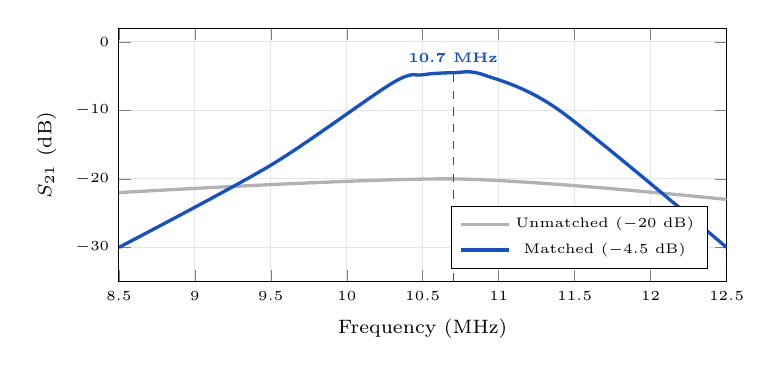
\begin{tikzpicture}
\begin{axis}[
  width=9.3cm, height=4.8cm,
  xlabel={Frequency (MHz)}, ylabel={$S_{21}$ (dB)},
  xmin=8.5, xmax=12.5, ymin=-35, ymax=2,
  grid=both, grid style={gray!20},
  tick label style={font=\tiny},
  label style={font=\scriptsize},
  legend style={font=\tiny,at={(0.97,0.05)},anchor=south east},
]
  \addplot[gray!60,very thick,smooth] coordinates{
    (8.5,-22)(10.7,-20)(12.5,-23)};
  \addlegendentry{Unmatched ($-20$ dB)}
  \addplot[ifcol,very thick,smooth] coordinates{
    (8.5,-30)(9.5,-18)(10.3,-6)(10.5,-4.8)
    (10.7,-4.5)(10.9,-4.8)(11.4,-10)(12.5,-30)};
  \addlegendentry{Matched ($-4.5$ dB)}
  \draw[ifcol,dashed,thin](axis cs:10.7,-35)--(axis cs:10.7,-4.5)
    node[above,font=\tiny,ifcol]{\textbf{10.7 MHz}};
\end{axis}
\end{tikzpicture}
\end{center}

\vspace{0.2cm}
\textbf{Smith chart: impedance matching journey}
\begin{center}
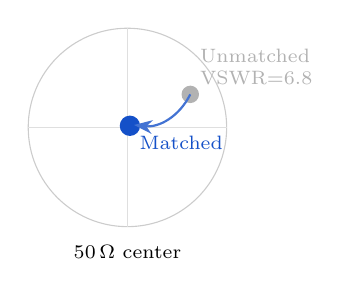
\begin{tikzpicture}[scale=1.05]
  \draw[gray!40](0,0) circle(1.2cm);
  \draw[gray!25,thin](-1.2,0)--(1.2,0);
  \draw[gray!25,thin](0,-1.2)--(0,1.2);
  \fill[gray!60](0.76,0.40) circle(3pt)
    node[above right,font=\scriptsize,align=left]{Unmatched\\VSWR=6.8};
  \fill[ifcol](0.03,0.02) circle(3.5pt)
    node[below right,font=\scriptsize,ifcol]{Matched};
  \draw[-Stealth,ifcol!80,thick,bend left=35](0.76,0.40) to (0.08,0.03);
  \node[font=\scriptsize] at (0,-1.5){50\,$\Omega$ center};
\end{tikzpicture}
\end{center}
\end{frame}

%% ── SLIDE 7: LAB 4 QUADRATURE I/Q ──────────────────────────────────────────
\begin{frame}{Lab 4 --- Quadrature I/Q Downconversion (1/2)}
\textbf{Three cascaded boards:}
\begin{enumerate}
  \item \textbf{ADT1-4W} transformer: $1\!:\!4$ impedance, SE $\to$ differential
  \item \textbf{74CBTLV3253}: quadrature analog switches\\
        Driven at $0^\circ/90^\circ/180^\circ/270^\circ$ by Si5351 CLK1/CLK2
  \item \textbf{AD4940-1} FDA: dual LPF + gain $= 2$
\end{enumerate}

\vspace{0.25cm}
\textit{\small Note: 74ALVC74 ($\div 4$) not used. Si5351 provides quadrature
directly via \texttt{set\_phase(CLK2,64)}.}

\vspace{0.35cm}
\textbf{Frequency math:}
\[
  f_\text{quad} = 10.95\text{ MHz}
\]
\[
  f_\text{low-IF} = |f_\text{IF} - f_\text{quad}|
  = |10.70 - 10.95| = \mathbf{250\text{ kHz}}
\]

\vspace{0.25cm}
\textbf{Measured result:}\\
I and Q outputs both show tone at 250 kHz.\\
C1: 5.45 V\textsubscript{pk-pk}, C2: 5.46 V\textsubscript{pk-pk} $\Rightarrow$ balanced amplitudes confirm $90^\circ$ phase relationship.
\end{frame}

\begin{frame}{Lab 4 --- Quadrature I/Q Downconversion (2/2)}
\textbf{I/Q phasor view}
\begin{center}
\begin{tikzpicture}[scale=1.25]
  \draw[-Stealth,gray!50](-1.6,0)--(1.6,0) node[right,font=\tiny]{Re};
  \draw[-Stealth,gray!50](0,-1.6)--(0,1.6) node[above,font=\tiny]{Im};
  \draw[-Stealth,ifcol,very thick](0,0)--(1.2,0)
    node[right,font=\small,ifcol]{I};
  \draw[-Stealth,bbcol,very thick](0,0)--(0,1.2)
    node[above,font=\small,bbcol]{Q};
  \draw[dashed,gray!50,thin](1.2,0) arc(0:90:1.2);
  \node[font=\scriptsize] at (0.55,0.55){$90^\circ$};
  \node[font=\tiny,gray] at (1.0,-0.2){$f_\text{BB}=250$ kHz};
\end{tikzpicture}
\end{center}

\vspace{0.2cm}
\textbf{Spectrum at baseband:}
\begin{center}
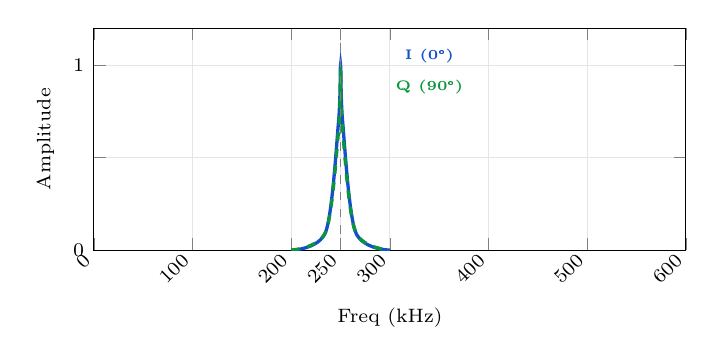
\begin{tikzpicture}
\begin{axis}[
  width=9.1cm, height=4.4cm,
  xlabel={Freq (kHz)}, ylabel={Amplitude},
  xmin=0, xmax=600, ymin=0, ymax=1.2,
  xtick={0,100,200,250,300,400,500,600},
  xticklabel style={rotate=45,anchor=east},
  ytick={0,0.5,1.0},
  yticklabels={0,,1},
  grid=both, grid style={gray!20},
  tick label style={font=\scriptsize},
  label style={font=\scriptsize},
]
  \addplot[ifcol,very thick,smooth] coordinates{
    (200,0)(235,0.1)(248,0.7)(250,1.0)(252,0.7)(265,0.1)(300,0)};
  \addplot[bbcol,very thick,smooth,dashed] coordinates{
    (200,0)(235,0.1)(248,0.65)(250,0.95)(252,0.65)(265,0.1)(300,0)};
  \node[ifcol,font=\tiny\bfseries] at (axis cs:340,1.05){I (0\textdegree)};
  \node[bbcol,font=\tiny\bfseries] at (axis cs:340,0.88){Q (90\textdegree)};
  \draw[dashed,gray,thin](axis cs:250,0)--(axis cs:250,1.2)
    node[above,font=\tiny]{250 kHz};
\end{axis}
\end{tikzpicture}
\end{center}
\end{frame}

%% ── SLIDE 8: EXPERIMENT 1 HARDWARE ─────────────────────────────────────────
\begin{frame}{Experiment 1 --- Quadrature + LPF: Hardware Validation (1/2)}
\begin{center}
{\large\bfseries Setup: ADT1-4W + 74CBTLV3253 + AD4940-1 LPF (no complex BPF)}\\[4pt]
{\normalsize IF = 10.7 MHz \quad $f_\text{quad}$ = 10.95 MHz \quad $\Rightarrow$ low-IF = \textbf{250 kHz}}
\end{center}

\vspace{0.2cm}
\centering
\textbf{Oscilloscope (I/Q waveforms)}

\vspace{0.15cm}
\includegraphics[width=0.83\textwidth,trim=0 20 0 20,clip]%
  {MatlabSimulations/plots/hw_quad_only.png}

\vspace{0.12cm}
{\small C1 (orange) = I channel \quad C2 (blue) = Q channel}\\
{\small Both at 250 kHz, balanced amplitudes $\approx$ 5.45 V\textsubscript{pk-pk}}
\end{frame}

\begin{frame}{Experiment 1 --- Quadrature + LPF: Hardware Validation (2/2)}
\begin{center}
{\large\bfseries Setup: ADT1-4W + 74CBTLV3253 + AD4940-1 LPF (no complex BPF)}\\[4pt]
{\normalsize IF = 10.7 MHz \quad $f_\text{quad}$ = 10.95 MHz \quad $\Rightarrow$ low-IF = \textbf{250 kHz}}
\end{center}

\vspace{0.2cm}
\centering
\textbf{Spectrogram (Digilent WaveForms)}

\vspace{0.15cm}
\includegraphics[width=0.83\textwidth]%
  {MatlabSimulations/plots/spec_quad_only.jpg}

\vspace{0.12cm}
{\small Tone at 250 kHz clearly visible in both channels.}\\[4pt]
{\small Both I and Q pass the desired tone --- image rejection not yet applied.}
\end{frame}

%% ── SLIDE 9: LABS A+B SIMULATION ───────────────────────────────────────────
\begin{frame}{Labs A+B --- Complex BPF \& MFB Adder: Simulation Results (1/2)}
\textbf{Single-path measurement (polyproc.m, esI/esQ)}\\
{\scriptsize Asymmetric response: desired pass vs image reject, + image rejection ratio:}

\vspace{0.1cm}
\begin{center}
\includegraphics[width=0.85\textwidth]%
  {MatlabSimulations/plots/polyphase_response.png}
\end{center}

\vspace{0.15cm}
\textbf{Full chain (ActProcB.m, espI/Q + esmI/Q)}\\
{\scriptsize Complex BPF + MFB adder two-sided response:}

\vspace{0.1cm}
\begin{center}
\includegraphics[width=0.85\textwidth]%
  {MatlabSimulations/plots/complex_bpf_full.png}
\end{center}
\end{frame}

\begin{frame}{Labs A+B --- Complex BPF \& MFB Adder: Simulation Results (2/2)}
\textbf{Lab A} --- Cross-coupled Tow-Thomas (4$\times$ THS4551)
\begin{itemize}
  \item Cross-coupled I/Q paths $\Rightarrow$ \textbf{asymmetric} frequency response
  \item Passes $-300$ kHz sideband (desired)
  \item Rejects $+300$ kHz sideband (image)
  \item Single path: $\approx \mathbf{43}$ dB rejection
\end{itemize}

\vspace{0.35cm}
\textbf{Lab B} --- MFB Adder (1$\times$ THS4551)
\begin{itemize}
  \item Combines I$'$ + Q$'$ into one real differential signal
  \item Full chain rejection: $\approx \mathbf{60}$ dB at 303 kHz
  \item Output feeds Lab C FM demodulator
\end{itemize}

\vspace{0.35cm}
\begin{center}
\begin{tabular}{ll}
\toprule
Path & Image Rej. \\
\midrule
Single path & $\approx$ 43 dB \\
Full chain  & $\approx$ \textbf{60 dB} \\
\bottomrule
\end{tabular}
\end{center}
\end{frame}

%% ── SLIDE 10: EXPERIMENT 2 HARDWARE ─────────────────────────────────────────
\begin{frame}{Experiment 2 --- Quad + Complex BPF + Adder: Hardware Validation (1/2)}
\begin{center}
{\large\bfseries Setup: Exp.\ 1 chain + Complex BPF (Tow-Thomas, 250 kHz) + MFB Adder}\\[4pt]
{\normalsize Expected: desired tone passes, image tone \textbf{suppressed by $\approx$ 60 dB}}
\end{center}

\vspace{0.2cm}
\centering
\textbf{Oscilloscope (after Complex BPF + Adder)}

\vspace{0.15cm}
\includegraphics[width=0.83\textwidth,trim=0 20 0 20,clip]%
  {MatlabSimulations/plots/hw_quad_cbpf.png}

\vspace{0.12cm}
{\small C1 (orange): tone at 250 kHz (desired) --- present}\\
{\small C2 (blue): image sideband --- \textbf{strongly suppressed}}
\end{frame}

\begin{frame}{Experiment 2 --- Quad + Complex BPF + Adder: Hardware Validation (2/2)}
\begin{center}
{\large\bfseries Setup: Exp.\ 1 chain + Complex BPF (Tow-Thomas, 250 kHz) + MFB Adder}\\[4pt]
{\normalsize Expected: desired tone passes, image tone \textbf{suppressed by $\approx$ 60 dB}}
\end{center}

\vspace{0.2cm}
\centering
\textbf{Spectrogram (after Complex BPF + Adder)}

\vspace{0.15cm}
\includegraphics[width=0.83\textwidth]%
  {MatlabSimulations/plots/spec_quad_cbpf.jpg}

\vspace{0.12cm}
{\small Desired tone at 250 kHz retained.}\\
{\small Image component greatly attenuated --- confirms $\approx 60$ dB rejection.}\\[4pt]
{\small \textbf{Compared to Exp.\ 1:} C2 now shows image suppression instead of equal amplitude.}
\end{frame}

%% ── SLIDE 11: LAB C + CONCLUSION ────────────────────────────────────────────
\begin{frame}{Lab C + Conclusion --- End-to-End FM Receiver (1/2)}
\textbf{Lab C --- FM Demodulation Board}
\begin{itemize}
  \item Inputs: In$+$, In$-$, VDD, GND (differential)
  \item FM discriminator: $\Delta f$ deviation $\to$ voltage
  \item Audio band recovered: 20 Hz -- 15 kHz $\to$ Speaker
\end{itemize}

\vspace{0.3cm}
\textbf{One station's journey (98.1 MHz):}

\vspace{0.1cm}
\small
\begin{tabular}{@{}lll@{}}
\toprule
Stage & In & Out \\
\midrule
Lab 0 LNA   & $-70$ dBm RF    & $-48$ dBm RF \\
Lab 2 Mixer & 98.1 + 87.4 MHz & 10.7 MHz IF \\
Lab 1 BPF   & mixed products  & 10.7 MHz clean \\
Lab 4 I/Q   & 10.7 MHz IF     & 250 kHz I/Q \\
Lab A CBF   & $\pm$250 kHz    & $-$250 kHz only \\
Lab B Adder & I$'$, Q$'$      & combined real \\
Lab C Demod & FM signal       & audio \\
\bottomrule
\end{tabular}
\end{frame}

\begin{frame}{Lab C + Conclusion --- End-to-End FM Receiver (2/2)}
\textbf{Key measurements:}
\begin{itemize}
  \item \textbf{LNA:} $+22$ dB gain, 2.3 dB NF (FM band, flat)
  \item \textbf{IF BPF:} $+15.5$ dB after L-network matching
  \item \textbf{Quadrature:} 250 kHz low-IF, balanced I/Q confirmed
  \item \textbf{Complex BPF:} $\approx 60$ dB image rejection
  \item \textbf{Audio:} recovered at speaker \checkmark
\end{itemize}

\vspace{0.3cm}
\textbf{Gain budget across chain:}
\begin{center}
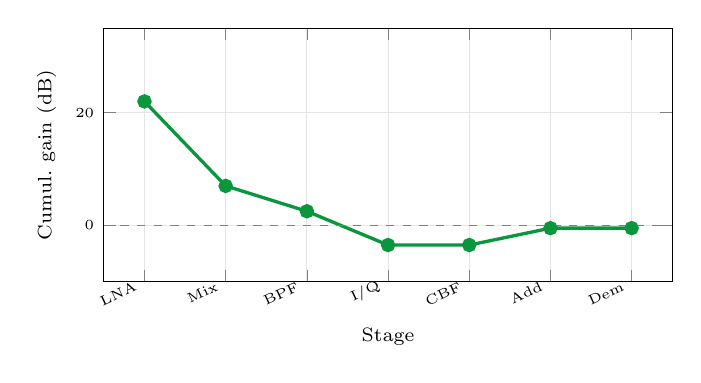
\begin{tikzpicture}
\begin{axis}[
  width=8.8cm, height=4.8cm,
  xlabel={Stage}, ylabel={Cumul.\ gain (dB)},
  xmin=0.5, xmax=7.5, ymin=-10, ymax=35,
  xtick={1,2,3,4,5,6,7},
  xticklabels={LNA,Mix,BPF,I/Q,CBF,Add,Dem},
  xticklabel style={rotate=25,anchor=east,font=\tiny},
  grid=both, grid style={gray!20},
  tick label style={font=\tiny},
  label style={font=\scriptsize},
]
  \addplot[bbcol,very thick,mark=*,mark size=2pt,
           mark options={fill=bbcol}] coordinates{
    (1,22)(2,7)(3,2.5)(4,-3.5)(5,-3.5)(6,-0.5)(7,-0.5)};
  \draw[dashed,gray,thin](axis cs:0.5,0)--(axis cs:7.5,0);
\end{axis}
\end{tikzpicture}
\end{center}

\vspace{0.15cm}
\begin{center}
\Large\textbf{\textcolor{bbcol}{Antenna $\longrightarrow$ Speaker}}\\[4pt]
\normalsize 88--108 MHz $\to$ 10.7 MHz $\to$ 250 kHz $\to$ audio
\end{center}
\end{frame}

\end{document}
